\section[Discriminating variable: $m_{\rm eff}$]{Discriminant variable: \boldmath{$m_{\rm eff}$}}
\label{sec:vlq:discrvar}
The separation between  the signal and background can be further increased exploiting the distinct kinematic features of the signal.  In the case of $T\bar{T}$ signal, the large $T$ quark mass results in leptons and jets with large energy in the final state. A powerful discriminating variable between signal and background can be build as the scalar sum of the transverse momenta of the lepton, the selected jets and the missing transverse momentum: the effective mass ($m_{\rm eff}$). In this case, the $m_{\rm eff}$ distribution peaks at approximately $2m_{T}$ for signal events and at lower values for the $t\bar{t}$+jets background. The different $t\bar{t}t\bar{t}$ signals, particularly those from BSM scenarios, also populate high values of $m_{\rm eff}$, whereas signals from associated heavy-Higgs boson production are typically softer in this variable. In the 1-lepton channel, an additional selection requirement of $m_{\rm eff} > 400$ $\gev$ ($m_{\rm eff} > 700$ \gev) is made for regions with exactly zero (one) mass-tagged jets, in order to minimise the effect of a possible mismodelling of the $m_{\rm eff}$ distribution at low values originating from small backgrounds with large systematic uncertainties, such as multijet production. This additional requirement on $m_{\rm eff}$ has no impact on the search sensitivity because the $T\bar{T}$ signal is characterised by having at least one mass-tagged jet and large values of $m_{\rm eff}$. Figure \ref{fig:vlq:discr:meff} compares the $m_{\rm eff}$ distribution between signal and background for events in two signal-rich regions of the 0-lepton and 1-lepton channels. The discrimination between signal and background becomes better with increasing $T$-quark masses. 


\begin{figure}[h!]
\begin{subfigure}{0.5\textwidth}
  \centering
  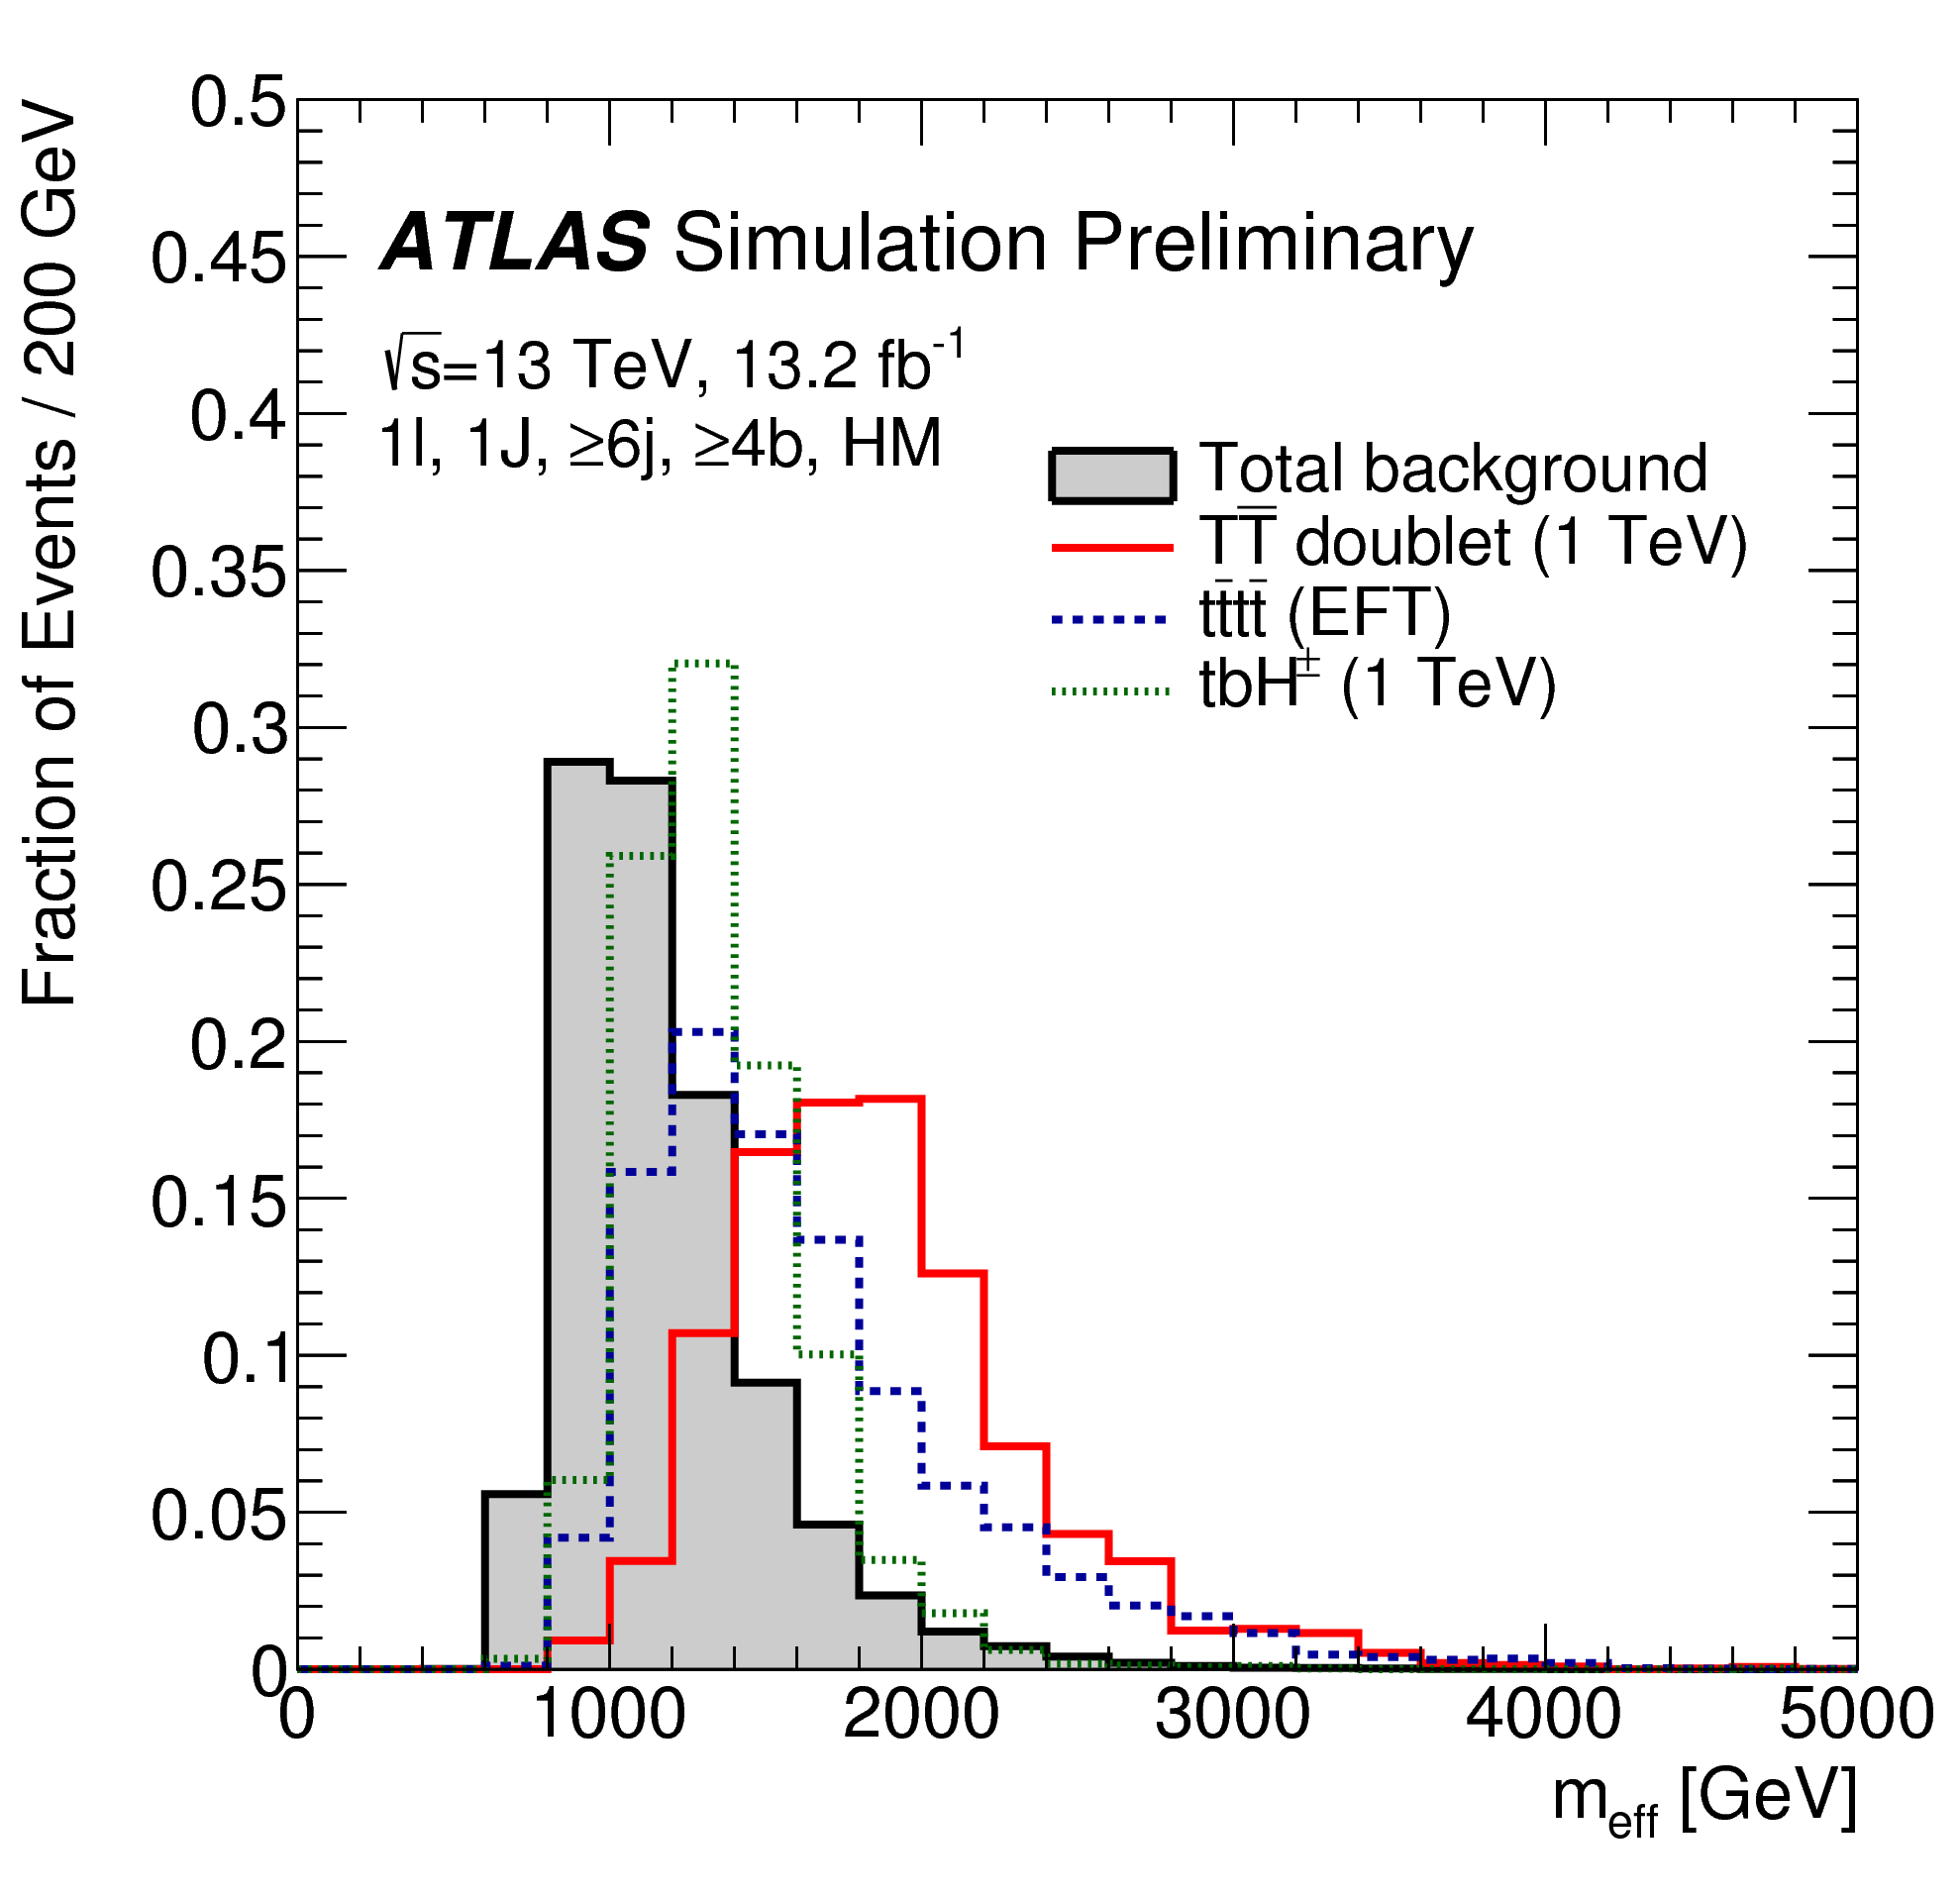
\includegraphics[width=0.9\textwidth]{figures/VLQ/meff1l.png}
  \caption{}
  \label{}
\end{subfigure}
\begin{subfigure}{0.5\textwidth}
  \centering
  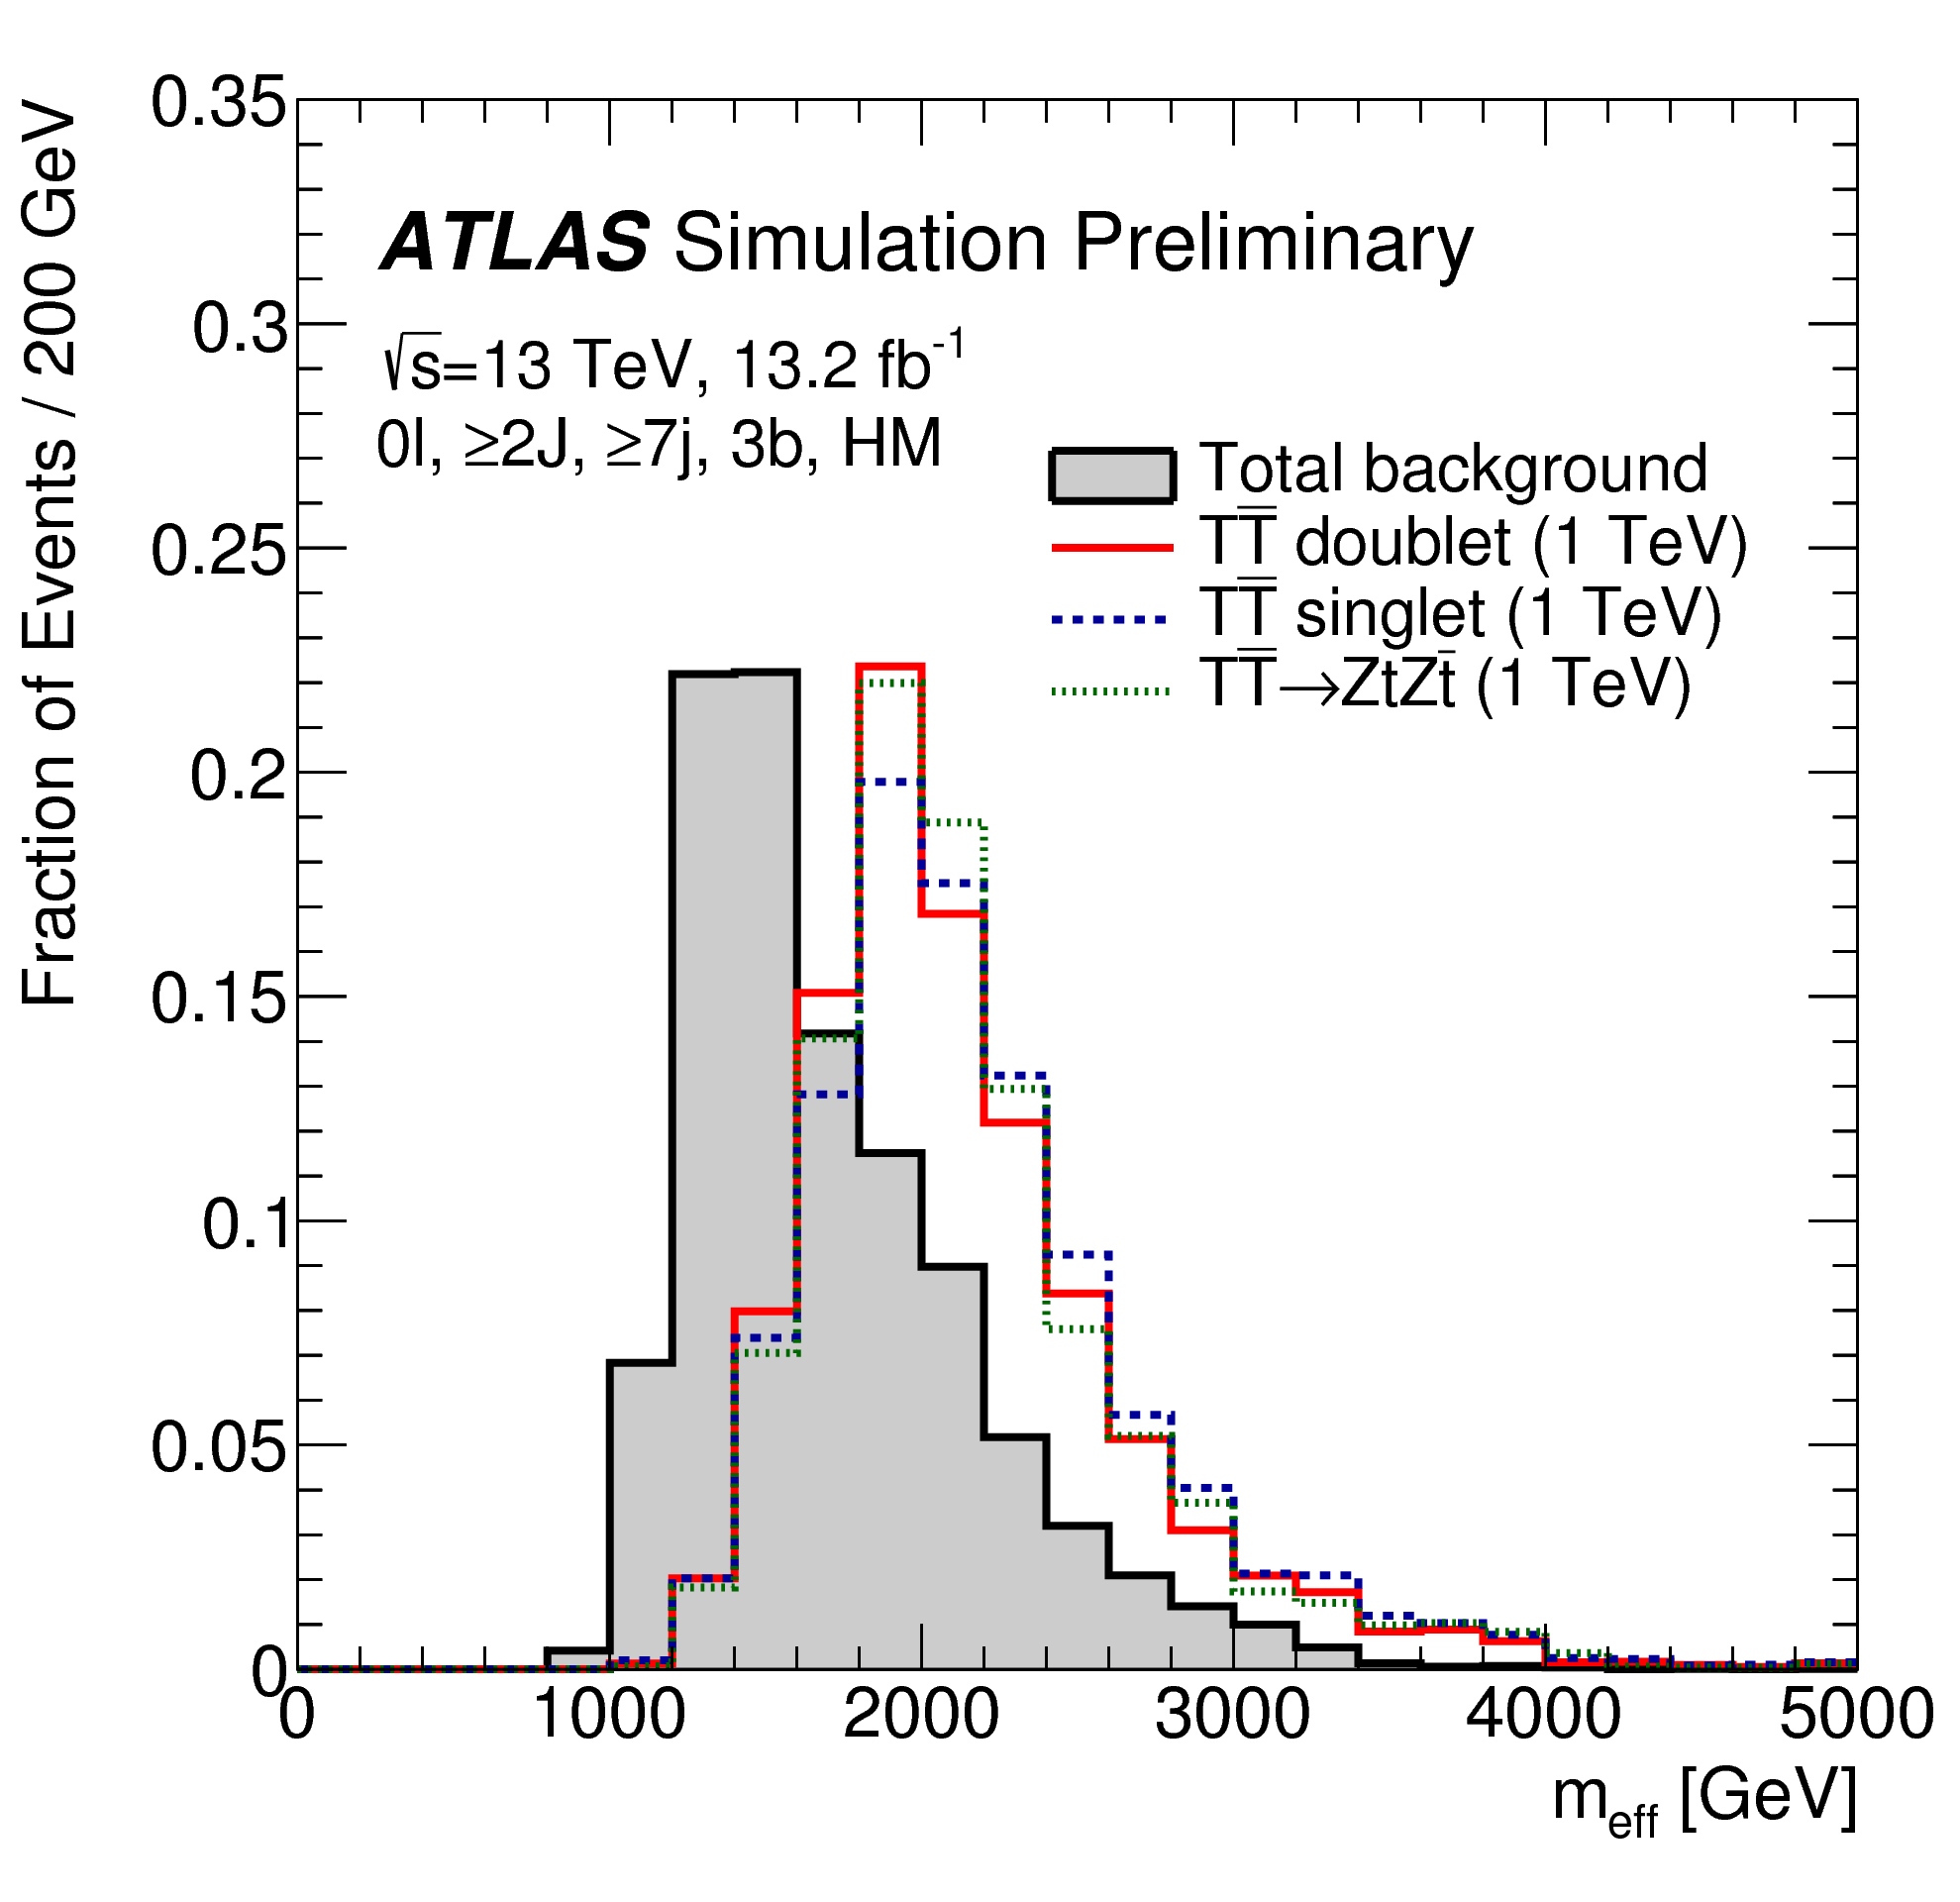
\includegraphics[width=0.9\textwidth]{figures/VLQ/meff0l.png}
  \caption{}
  \label{}
\end{subfigure}

\captionsetup{width=0.85\textwidth} \caption{\small Comparison of the shape of the distribution of the scalar sum of the transverse momenta of the lepton, the selected jets and the missing transverse momentum ($m_{\rm eff}$) between the total background (shaded histogram) and several signal scenarios considered in this search. The signals shown are: $T\bar{T}$ production in the weak-isospin doublet and singlet scenarios, and for ${\rm BR}(T\to Zt) = 1$, assuming $m_{T} = 1$ \tev; $t\bar{t}t\bar{t}$ production within an EFT model; and $tbH^{\pm}(\to tb)$ production assuming $m_{H^{\pm}} = 1$ \tev. The selection used in (a) corresponds to events in the (1J, $\ge$6j, $\ge$4b, HM) region of the 1-lepton channel, whereas the selection used in (b) corresponds to events in the ($\ge$2J, $\ge$7j, 3b, HM) region of the 0-lepton channel. The last bin in both figures contains the overflow.}
\label{fig:vlq:discr:meff}
\end{figure}